\documentclass[14pt, a4paper]{extarticle}
\usepackage{extsizes}
\usepackage[T2A,T1]{fontenc}
\usepackage[utf8]{inputenc}
\usepackage{biblatex}
\usepackage{hyperref}
% \usepackage{mwe}
\usepackage{blindtext}
\usepackage{wrapfig}
\usepackage{multicol}
\usepackage{xcolor}
\usepackage[utf8]{inputenc}
\usepackage{graphicx}
\usepackage{setspace}
\usepackage{float}
\usepackage{newtxtext, newtxmath}
\usepackage{amsmath}
% \usepackage{lmodern}

% A flag to turn on "fancy" compilation - no stuff related to my university
% \def \fancy
\graphicspath{ {./assets/} }

\bibstyle{plain}
\bibliography{main.bib}

\begin{document}
\ifx\fancy\undefined{}
	%
% This titlepage is used for HSE internal report only
%

\begin{titlepage}
    \begin{center}
          \textbf{\MakeUppercase{National Research University\\ Higher School of Economics}}

          \vspace*{1cm}

          Faculty of Computer Science\\
          Bachelor's Programme `Data Science and Business Analytics'
    \end{center}

    % TODO FIXME %
    UDC \underbar{\hspace{3cm}}

    \vspace*{1.5cm}

    \center{\textbf{Research Project Report}}\\
    On the topic `Topological and Geometric Deep Learning'

    \vspace*{2cm}

    \begin{flushleft}
        \textbf{Fulfilled by the Student:}\\
        Chechulin Nikolay Dmitrievich, Signature: \underbar{\hspace{3cm}}\\
        Group DSBA-201
        
        \vspace*{1cm}
        
        \textbf{Checked by the Project Supervisor}\\
        Kachan Oleg Nikolaevich,\\
        Research assistant at International Laboratory for Applied Topology and Applications

        \today \hspace*{1cm}\\
        Grade: \underbar{\hspace{1.5cm}} \hspace*{1cm}
        Signature: \underbar{\hspace{3cm}}

    \end{flushleft}

    \vfill
    \textbf{Moscow, 2022}
\end{titlepage}

\else
	\graphicspath{ {./assets/} }

\begin{titlepage}
	\begin{center}
		\vspace*{1cm}

		{\huge \textbf{Topological and geometric deep learning}}

		\vspace{0.5cm}
		%   {\large TODO FIXME }

		\vspace{1.5cm}

		{\large Student: \textbf{Nikolay Chechulin}, DSBA-201}

		{\large Academic Supervisor: \textbf{Oleg Kachan}}

		\vfill
		\vspace{1.5cm}

		
\includegraphics[width=0.4\textwidth]{Higher_School_of_Economics_Logo}

		Faculty of Computer Science\\
		Bachelor's programme `Data Science and Business Analytics'\\
		Moscow, Russia\\
		2022

	\end{center}
\end{titlepage}

\fi

\begin{abstract}
	Nowadays, a need to analyze more complex data arises.
	Some objects and relations can not be represented as vectors in Euclidean space, and, therefore, we have to consider graphs --- sets of nodes and connections between them --- as a subject of analysis.
	They are able to hold more information than traditional Euclidean object --- for example, nodes and edges may have their own features.
	It is also possible to extract topological information from a graph --- by determining its `shape' we can understand the relation between nodes and somehow make use of this information.

	This poses a huge problem: we have to invent new algorithms, adapt known techniques and constantly improve them in order to work with such a complex data.
	Our goal is to research the efficiency of several tweaks of existing models and means of preprocessing graphs in order to increase several key indicators.
\end{abstract}
\pagebreak

\tableofcontents

\section{Introduction}

\subsection{Abstract}
    Nowadays, a need to analyze more complex data arises.
    Some objects and relations can not be represented as vectors in Euclidean space, and, therefore, we have to consider graphs --- sets of nodes and connections between them --- as a subject of analysis.
    They are able to hold more information than traditional Euclidean object --- for example, nodes and edges may have their own features.
    It is also possible to extract topological information from a graph --- by determining its `shape' we can understand the relation between nodes and somehow make use of this information.

    This poses a huge problem: we have to invent new algorithms, adapt known techniques and constantly improve them in order to work with such a complex data.
    Our goal is to research the efficiency of several tweaks of existing models and means of preprocessing graphs in order to increase several key indicators. 
    
\subsection{Relevance}
    The field of research (graph neural networks) might be considered relatively new, and, therefore, there is a huge number of possible improvements to be made to existing models and approaches.
    Our ultimate goal is to improve the accuracy of node and graph classification.

    For example, one of the proposed changes is to modify a Laplacian in such a way that it does not break existing model and improves it.
    Our initial results have shown that our approach indeed works well on Karate club dataset, where we had to classify nodes:

    \begin{figure}[h]
        \centering
        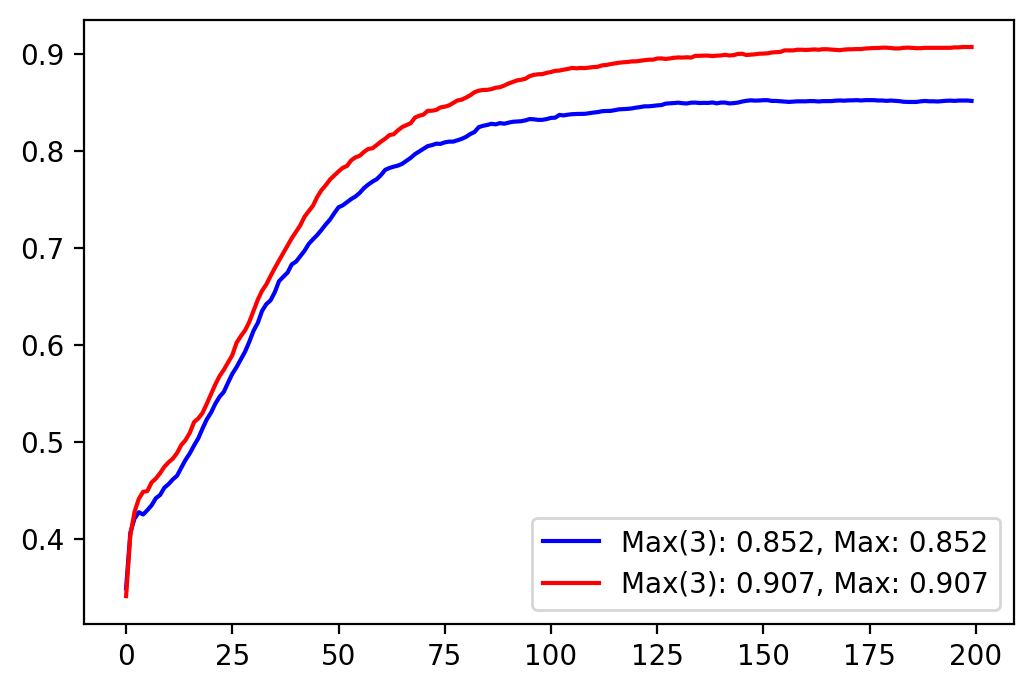
\includegraphics[width=0.6\textwidth]{custom_laplacian_accuracy.jpg}
        \caption{Default Laplacian (in blue) versus our Laplacian (in red). Y-axis is the accuracy, X-axis is the number of epochs}
    \end{figure}

    The relative novelty of the field allows us to find new experiments and techniques.

\subsection{Subject of research}
Let us explain the tasks we can solve using GNNs \emph{Graph Neural Networks} in more detail.
    There are three of them:
    \begin{itemize}
        \item \textit{Node classification} --- given a graph with several labelled nodes and several classes predict a class of an unlabelled node.
            For example, the CORA~\cite{cora_dataset} contains information about scientific papers.
            Each paper belongs to exactly one of seven given classes.
            Our task is to determine the class of a new paper given its feature vector and connections with other papers (in this case the edges of the graph are citations, the edges are undirected).
        \item \textit{Graph classification} --- determine type of graph.
            A good example of this task is presented classification of molecules~\cite{how_powerful_are_gnns} or image classification~\cite{benchmarking_gnns}, as well as in many other fields.
        \item \textit{Link prediction} --- determine if two given nodes should have an edge between them.
            A simple example could be friends suggestions in a social network.
    \end{itemize}

    In our research we will only consider the first two problems.

    As we established, we want to consider several changes in order to improve the accuracy.
    The tweaks we propose include but are not limited to:
    \begin{itemize}
        \item \textit{Altering the way we compute Laplacian} --- a characteristic matrix of a graph.
        \item \textit{Edge embeddings}
        \item \textit{Using connectivity over simplices of higher dimension}. This means that in some cases we might want to consider a group of nodes as a separate object, therefore, increasing the connectivity factor. We will only work with 3-simplices:
            \begin{figure}[h]
                \begin{multicols}{2}
                    \centering
                    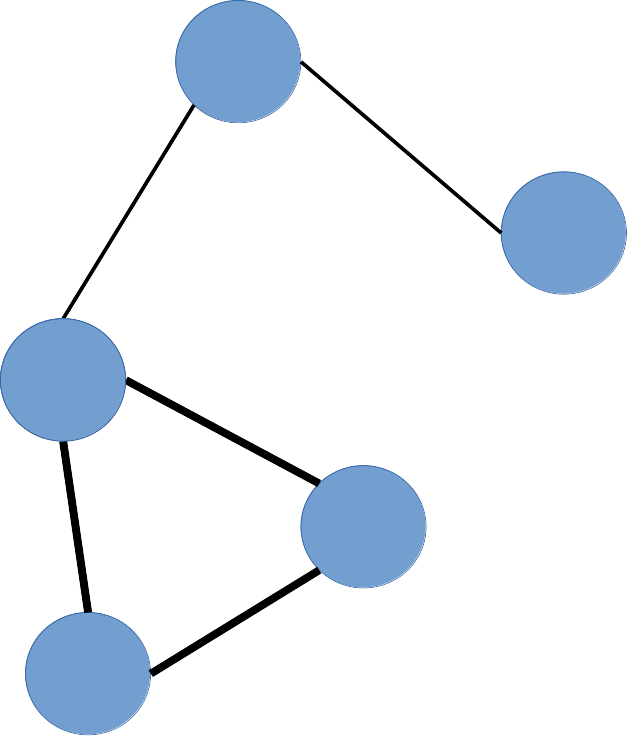
\includegraphics[width=0.2\textwidth]{simplex_1.png}
                    \caption{A part of some graph}\label{fig:clique_merged}
        
                    \centering
                    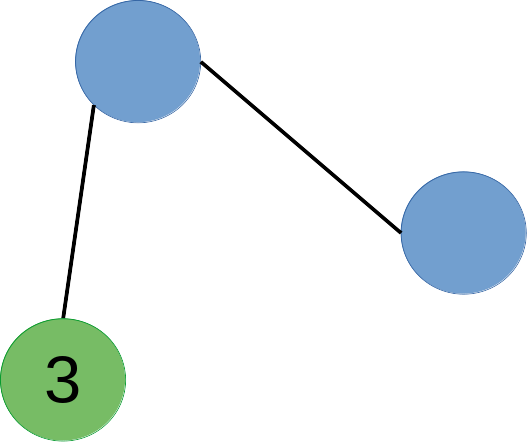
\includegraphics[width=0.2\textwidth]{simplex_2.png}
                    \caption{Three nodes from the left image united in 3-simplex having properties of the initial vertices}
                \end{multicols}
            \end{figure}
    \end{itemize}


\section{Definitions}

\subsection*{Graph}
\addcontentsline{toc}{subsection}{Graph}

Graph is a tuple $\left( V, E \right)$, where $V$ is the set of all nodes $v$, and $E$ is the set of edges $e_i = (v_j, v_k)$.

Graphs can be undirected ($(v_j, v_k) \equiv (v_k, v_j)$) and directed, where presence of the edge $(v_j, v_k)$ does not imply that edge $(v_j, v_j)$ exists.
Edges can also have weights which show some information about the tightness of connection of two nodes.
In this case $e_i = (v_j, v_k, w_i)$.

For instance, a road map of a country is an undirected weighted graph, where cities are nodes, roads are edges, and distances are weights.


\subsection*{Clique}
\addcontentsline{toc}{subsection}{Clique}

A graph clique is a subset of its nodes such that it is fully connected.
So, n-clique is a set of $n$ nodes and $\frac{n \cdot (n - 1)}{2}$ edges~\cite{wiki_clique}.

We will work mainly with 3-cliques, and often will refer to them as triangles.

\begin{figure}[H]
	\centering
	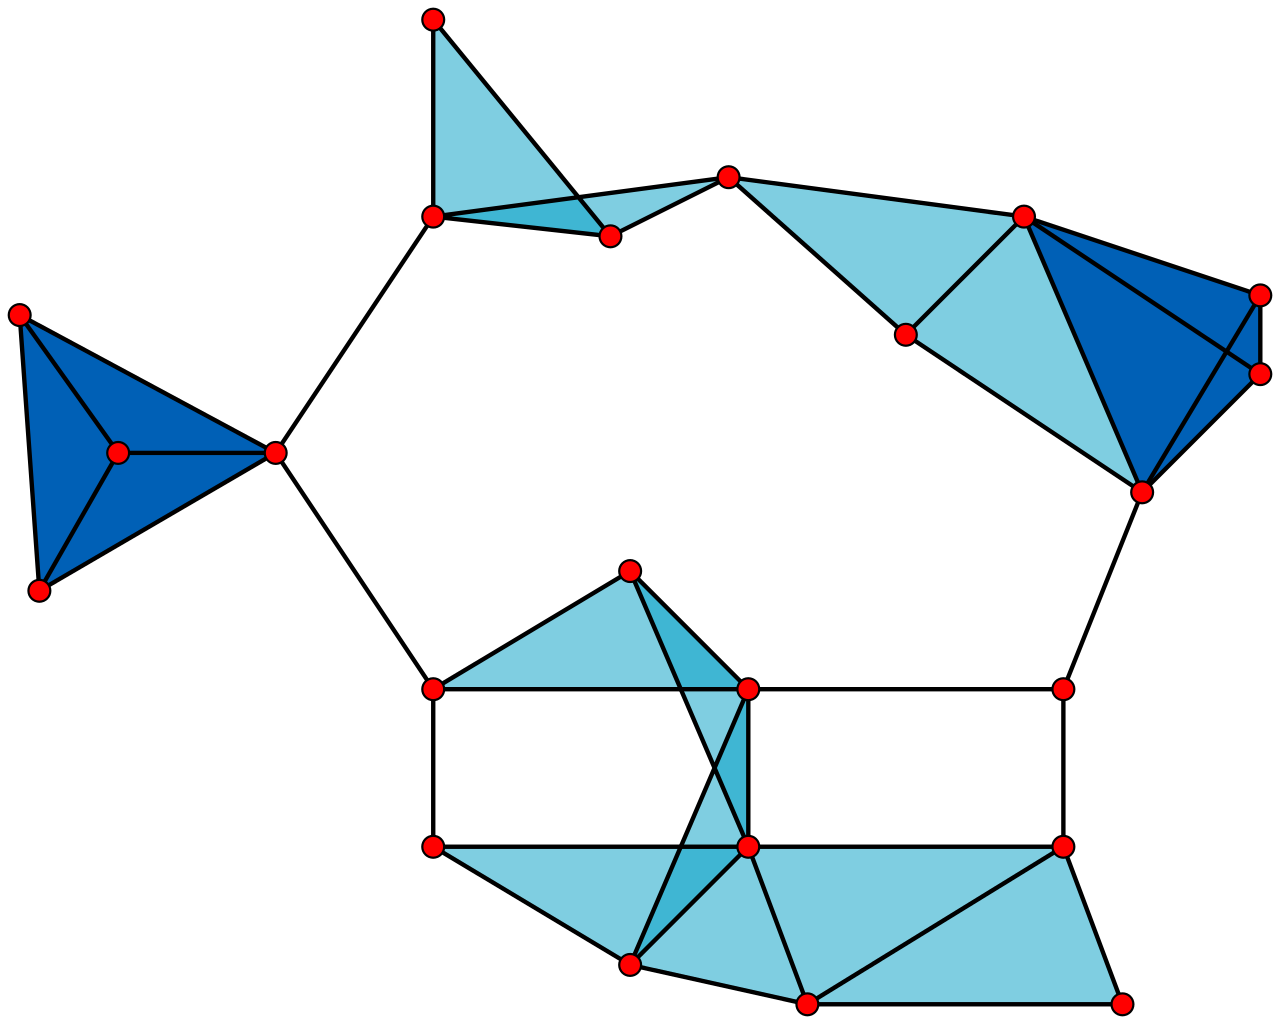
\includegraphics[width=0.8\textwidth]{clique.png}
	\caption{A graph with 23 1-vertex cliques (the vertices), 42 2-vertex cliques (the edges), 19 3-vertex cliques (light and dark blue triangles), and 2 4-vertex cliques (dark blue areas).}
\end{figure}


\subsection*{Adjacency Matrix}
\addcontentsline{toc}{subsection}{Adjacency Matrix}

$\lvert V \rvert \times \lvert V \rvert$ adjacency matrix $A$ is defined as follows: $A_{i, j} = 1$ if there is an edge from $v_i$ to $v_j$.
In our project we will consider undirected graphs with self-loops.
This means that $\forall i, j\ A_{i, j} = A_{j, i}$ and $\forall i\ A_{i, i} = 1$.


\subsection*{Incidence Matrix}
\addcontentsline{toc}{subsection}{Incidence Matrix}

If we have an undirected graph $(V, E)$, its incidence matrix $\nabla$ of size $\lvert V \rvert \times \lvert E \rvert$ such that $A_{i, j} = 1$ if $i$-th vertex is a vertex of $j$-th edge.
In directed case, we mark the initial vertex as -1, and the terminal as 1~\cite{wiki_incidence}.

\begin{multicols}{2}
	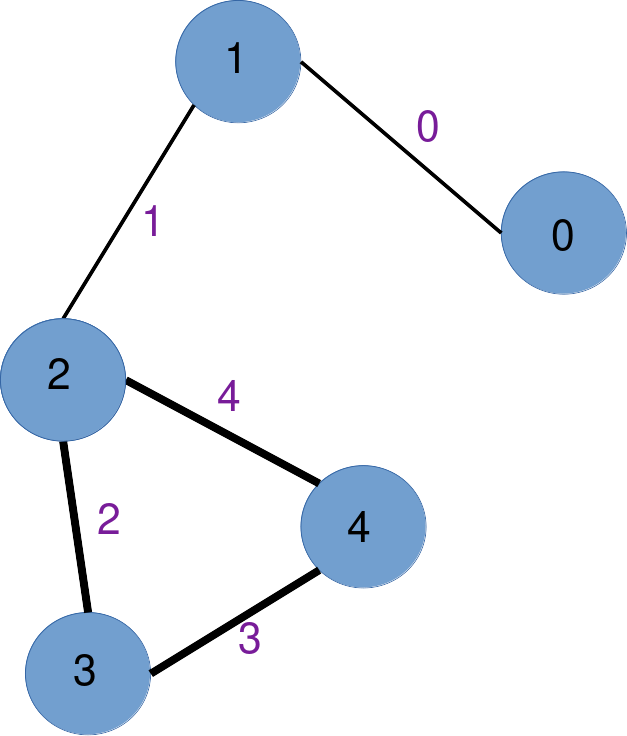
\includegraphics[width=0.3\textwidth]{incidence.png}

	The incidence matrix of the graph on the left would be as follows:

	\[
		\begin{bmatrix}
			1 & 0 & 0 & 0 & 0 \\
			1 & 1 & 0 & 0 & 0 \\
			0 & 1 & 1 & 0 & 1 \\
			0 & 0 & 1 & 1 & 0 \\
			0 & 0 & 0 & 1 & 1 \\
		\end{bmatrix}
	\]

\end{multicols}


\subsection*{Degree Matrix}
\addcontentsline{toc}{subsection}{Degree Matrix}

$\lvert V \rvert \times \lvert V \rvert$ diagonal degree matrix $D$ is defined as follows: $D_{i,i} = \Sigma_j A_{i, j}$ (that is, $D_{i, i} = in\_degree(v_i) + out\_degree(v_i)$)


\subsection*{Laplacian matrix}
\addcontentsline{toc}{subsection}{Graph Laplacian}

\textbf{Laplacian matrix} --- A matrix representation of a graph.
Usually is calculated using the following formula~\cite{wiki_laplacian}:
\begin{equation*}
	L_{i, j} =
	\begin{cases}
		\deg(v_i) & \mbox{if}\ i = j                                                 \\
		-1        & \mbox{if}\ i \neq j\ \mbox{and}\ v_i \mbox{ is adjacent to } v_j \\
		0         & \mbox{otherwise},
	\end{cases}
\end{equation*}

However, other definitions also take place: $L = D - A$, where $D$ is a degree matrix and $A$ is an adjacency matrix.
Another way to calculate a Laplacian is $L = \nabla\nabla^{T}$, where $\nabla$ is an incidence matrix.


\subsection*{Convolutional Graph Network}
\addcontentsline{toc}{subsection}{Convolutional Graph Network}

\textbf{CGN} \textit{(Convolutional Graph Network)} --- A type of GNN which generalizes the convolution operation to graphs.
Often we encounter convolution while we work with grid-structured data like images, but here we use same idea (aggregate features of the neighbors) on nodes instead of pixels~\cite{Wu_Pan_Chen_Long_Zhang_Yu_2021}~\cite{Kipf_Welling_2017}.

\begin{figure}[h]
	\begin{multicols}{2}
		\centering
		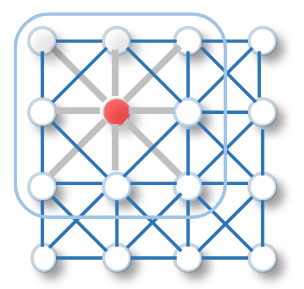
\includegraphics[width=0.4\textwidth]{conv.png}
		\caption{Convolution on image}

		\centering
		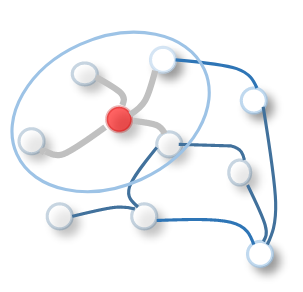
\includegraphics[width=0.4\textwidth]{CGN_conv.png}
		\caption{Convolution on graph}
	\end{multicols}
\end{figure}

Assume we have a graph of $N$ nodes, where each node has $F$ features.
We can construct an $N \times F$ matrix called feature matrix.
The first layer takes the feature matrix, and performs the following operation: $Z = D^{-\frac{1}{2}} A D^{-\frac{1}{2}} X W$, where:
\begin{itemize}
	\item $Z$ is resulting $N \times C$ signal
	\item $D$ is $N \times N$ degree matrix
	\item $A$ is $N \times N$ adjacency matrix with self-loops
	\item $X$ is $N \times F$ feature matrix (input signal)
	\item $W$ is $F \times C$ learnable weight matrix
\end{itemize}

Then the output $Z$ is directed into next layer, which does practically the same.
There might be many convolutional layers, but usually models only have 2.

The last (output) layer usually applies softmax function to each row resulting in a new matrix $S$.
Then, in order to classify a node $v_i$ we simply take the index of maximum of $S_i$.

The architecture of a graph convolutional network is presented on the figure below~\cite{simplifying_gcn}
\begin{figure}[h]
	\centering
	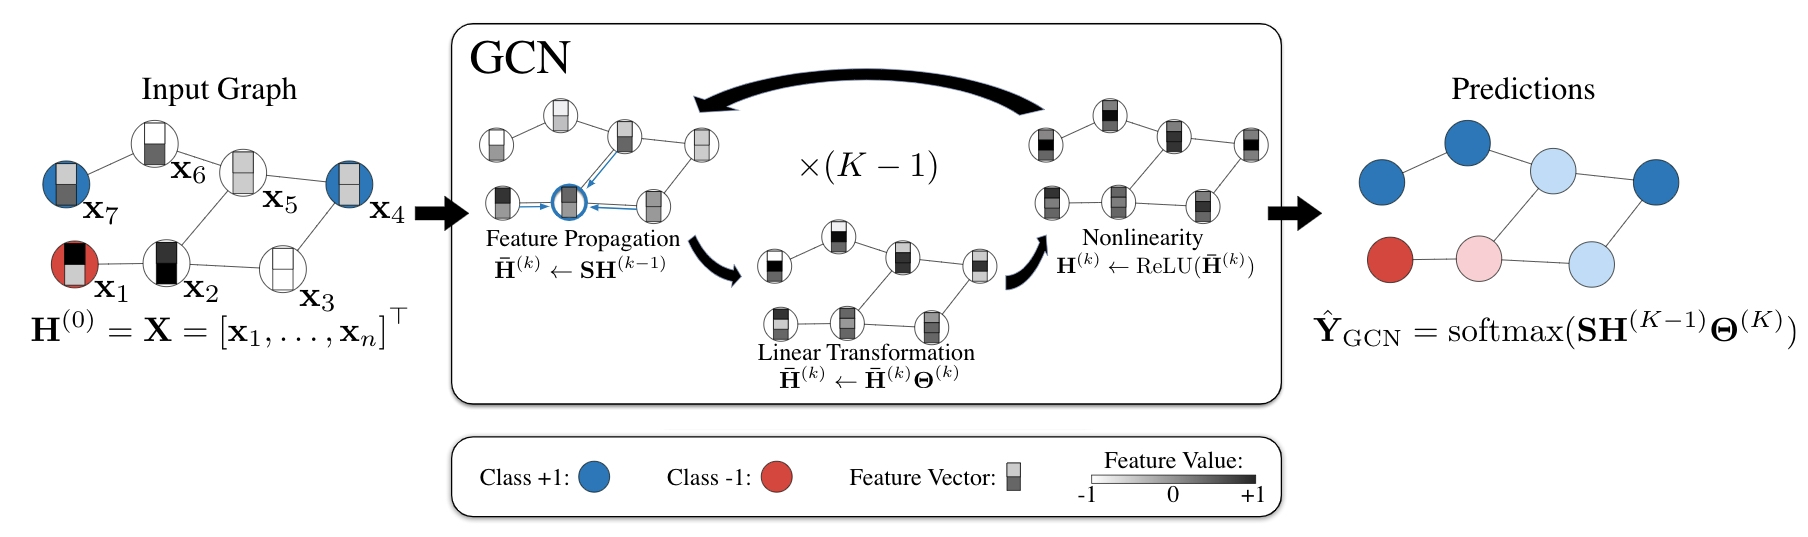
\includegraphics[width=0.9\textwidth]{gcn.jpg}
	\caption{Architecture of a GCN}
\end{figure}

\subsection*{Graph Attention Network}
\addcontentsline{toc}{subsection}{Graph Attention Network}

\textbf{GAT} \textit{(Graph Attention Network)} --- A type of GNN which uses attention mechanism (also borrowed from `casual' neural networks) which allows us to work with inputs of variable sizes and to focus on the most important features~\cite{Veličković_Cucurull_Casanova_Romero_Liò_Bengio_2018}.
The attention mechanism is a function $a: \mathbb{R}^C \times \mathbb{R}^C \rightarrow \mathbb{R}$ which takes two feature vectors $X_i, X_j$ and returns a scalar representing how tight the connection between $v_i$ and $v_j$ is.

We introduce an $N \times N$ matrix $e$ storing the attention between the nodes: $e_{i, j} = a\left( W \cdot X_i,\ W \cdot X_j \right)$.
Now we have to be careful about choice of $i$ and $j$, since if we calculate the attention between all the nodes, we will completely drop structural information of the graph.
One suggested solution is to use a neighborhood $\mathcal{N}_i$ of a vertex $v_i$ and then compute $e_{i, j}$ for all $j \in \mathcal{N}_i$.
Existing model~\cite{Veličković_Cucurull_Casanova_Romero_Liò_Bengio_2018} uses neighborhood of size 1 (that is, $v_i$ itself and all of its neighbors $v_j$ such that $\exists e = (v_i, v_j)$), and it seems to perform great.

One might also want to normalize the coefficients.
In order to do that, we can apply softmax function: $c_{i, j} = \text{softmax}_j \left( e_{i, j} \right) = \frac{\text{exp} \left( e_{i, j} \right)}{\Sigma_k \text{exp} \left( e_{i, k} \right) }$.

\begin{figure}[h]
	\centering
	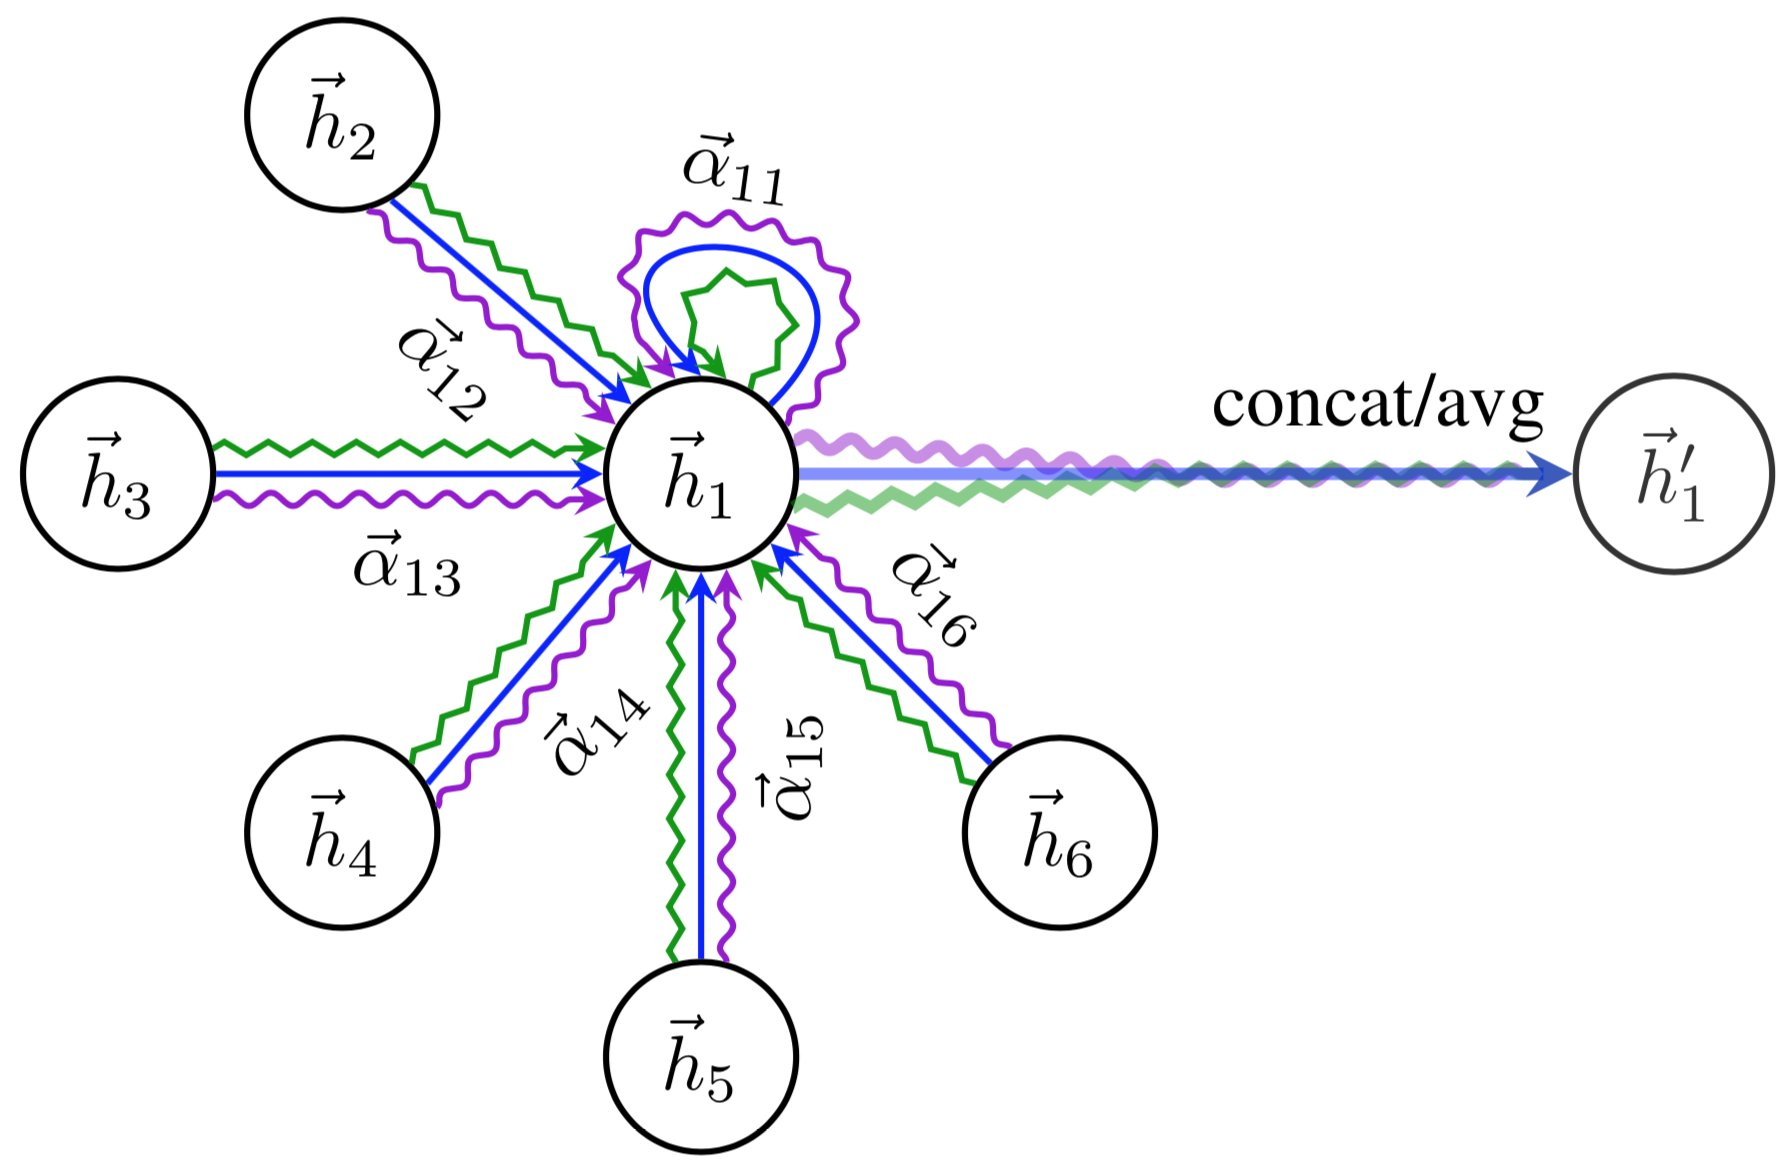
\includegraphics[width=0.7\textwidth]{gat.jpeg}
	\caption{An example of multi-head attention in a neighborhood of size 1}
\end{figure}




%\ifx\fancy\undefined{}
%    \section{Work schedule}

\subsection{Done}

At this point, I have understood the subject area by thoroughly reading the papers mentioned in the reference section.
Also, I started implementing my own implementation of a Graph Convolutional Network from scratch (that is, without any frameworks at all)~\cite{gcn_implementation}.

We made this decision in order to be able to dig even deeper into the topic.
Another benefit is the fact that improves the flexibility, since it is much easier to experiment with code written by yourself, rather than try to modify existing models.

\subsection{Future plans}

\begin{enumerate}
	\item \textit{Finish implementing the model}.
	      It still lacks some crucial modules to work, however, we are almost at the finish line.
	      The only part missing at the moment is the backpropagation logic.
	      This should be done by the end of February 2022.

	\item \textit{Find additional datasets}.
	      There are several datasets which are used for benchmarks~\cite{cora_dataset}~\cite{karate_club_dataset}, however, it is always great to find new ones in order to see how existing models perform and how our tweaks influence the results.
	      This is an ongoing task, so it does not have a particular deadline.

	\item \textit{Generalization of Laplacian}.
	      Extraordinary simple to implement as soon as our model is done, but requires some time finding the generalizations.

	\item \textit{Work with simplices of higher dimensions}.
	      This requires development of some kind of preprocessing mechanism, which takes graph as an input and provides the neural network with another graph.
	      Efficiency is important, so the development might take significant time.
	      I estimate the deadline to be in the middle of March 2022.

	\item \textit{Come up with new experiments}
\end{enumerate}
%\fi

\section{Experiments}
\newcommand\abs[1]{\ensuremath{\lvert #1 \rvert}}

\subsection{3-Clique merge with insertion}

\subsubsection*{Description}

In this experiment we find all the 3-cliqes~\cite{wiki_clique} (triangles) in the graph, then sort them based on `distance' and replace each 3-clique with one node sharing the features of the initial three.

The source code is available in the project repository and can be found in the `experiments' directory~\cite{3clique_ins_experiment}.

\subsubsection*{Algorithm}

Firstly, let us define a 3-clique more formally.
We define it as follows: $
\{ \left(a, b, c\right)\ 
\lvert\ a, b, c \in V \wedge
\left(a, b\right),
\left(a, c\right),
\left(b, c\right) \in E \} $.

While merging nodes in the cliques, we might face a problem: some of the nodes might participate in several 3-cliques.
In order to solve it, we need to introduce a mechanism for ordering cliques so that we could show preference to one instead of the other.
Naturally, such a mechanism should rely on the nodes feature vectors.
There are 2 major distance calculating algorithms: Euclidean distance and Manhattan distance.
Since the feature vectors are very sparse, the algorithms give quite close results and there is no need to consider them separately.

Using Euclidean distance we can map each 3-clique into a real number by calculating the sum of pairwise distances: $\abs{a_f - b_f}^2 + \abs{a_f - c_f}^2 + \abs{b_f - c_f}^2$, where $v_f$ stands for node's $v$ feature vector.
The resulting ordering now allows us to choose one 3-clique instead of another, since we know that one has its nodes `closer' to each other.

Therefore, one can simply sort all the 3-cliques in ascending order, merge each 3-clique and filter out all the `later' 3-cliques containing nodes from the current one.
This allows us pick the closest and most valuable nodes in a greedy way while also saving us from using a `new' node in another 3-clique ($(a, b, c) \rightarrow a';\ (a', d, e) \rightarrow a''$ is not allowed, since the graph could collapse).

\begin{enumerate}
    \item Find all the 3-cliques in graph.
    \item Sort them according to the sum of distances between nodes
    \item Merge all `valid' 3-cliques in one node preserving all the edges coming in and out of the triplet filtering out all the cliques containing nodes from the merged ones
    \item Generate new dataset from the resulting graph
\end{enumerate}

The process is shown on Figure~\ref{fig:clique_merged}.

\subsubsection*{Results and interpretation}

A benchmark on the Cora dataset~\cite{cora_dataset} had shown that we are able to remove a total of 12.2\% of nodes (the number reduced from 2708 to 2378) and 42.3\% edges (from 10556 to 6094).
Since the operation of merging of all cliques fast comparing to the model's learning time, we reduced the latter approximately by 23\%.
This improvement can be also seen on the loss graph of our models:

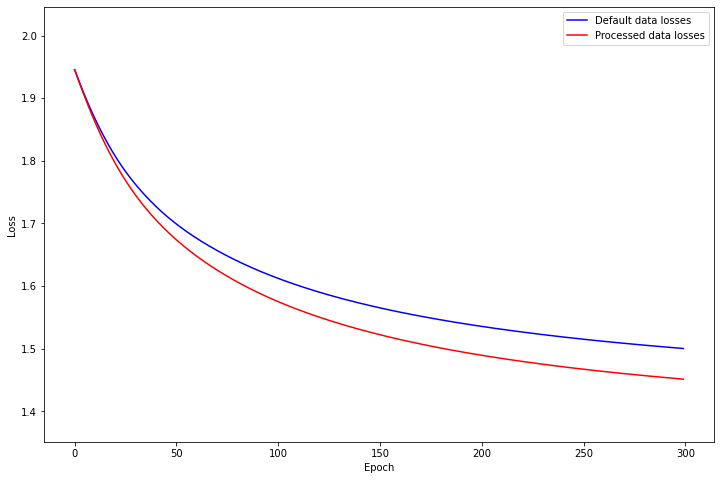
\includegraphics[width=0.9\textwidth]{3clique_loss.png}

Speaking of accuracy, we claim it did not change much.
On average, the accuracy of a default model lies somewhere between 0.7 and 0.75 and the model with 3-cliques merged performs practically same with an error of $\pm 0.01$ (for example, 0.725 vs 0.72402).

Therefore, we can claim that the only purpose of merging 3-cliques is reducing the learning time without any loss of accuracy.
It doesn't make much sense for theoretical purposes, however, is definitely an advantage in production.

\subsection{Graph of merged 3-cliques}

\subsubsection*{Description}

This experiment is very similar to the previous one.
The only difference is the resulting graph: in the first experiment we inserted the merged cliques back into the graph, but now we will erase all the nodes which are not a merged 3-clique.

\subsubsection*{Algorithm}
\subsubsection*{Results and interpretation}

\printbibliography{}
\end{document}
